\section{Introducing \em{Via}}
\label{sec:viaIntro}

Here we introduce the minimum of underlying computation that is needed
to understand {\em Via} graphs. Details follow in
Section~\secref{sec:methodology}.

We use student data from a large US private research university. This
dataset contains the anonymized enrollment data of over 52,000
students who were enrolled at the university during any time between
Fall 2000 and Fall 2018. Each of the roughly two million rows in this
table consists of a unique student identifier, a course in which they
enrolled, and the academic term during which they enrolled in the
class. The dataset also contains supplementary information, including
each student's major during time of enrollment in a course and each
student's major upon graduation.

Depending on the class of problems of interest, we filter along these
additional values. Similar filters could be used with {\em Via} over
demographic data that are available to university administrators. We
did not have such data available, but hope that our examples below
suggest the significant additional potential for {\em Via} to inform
understanding of gender, first-generation, ethno-racial minority status or other relevant subgroup characteristics.

{\em Via} converts course enrollment data to directed graphs.
Nodes represent courses, directed links represent sequential
enrollment in the courses at the link endpoints. Link weights model
conditional probabilities of enrolling in the link destination course,
given prior enrollment in the course at the link origin. Link weights
are visualized as line thickness.

{\em Via} partitions the graphs by the departments with which courses
are associated. 

\begin{figure}
    \centering
    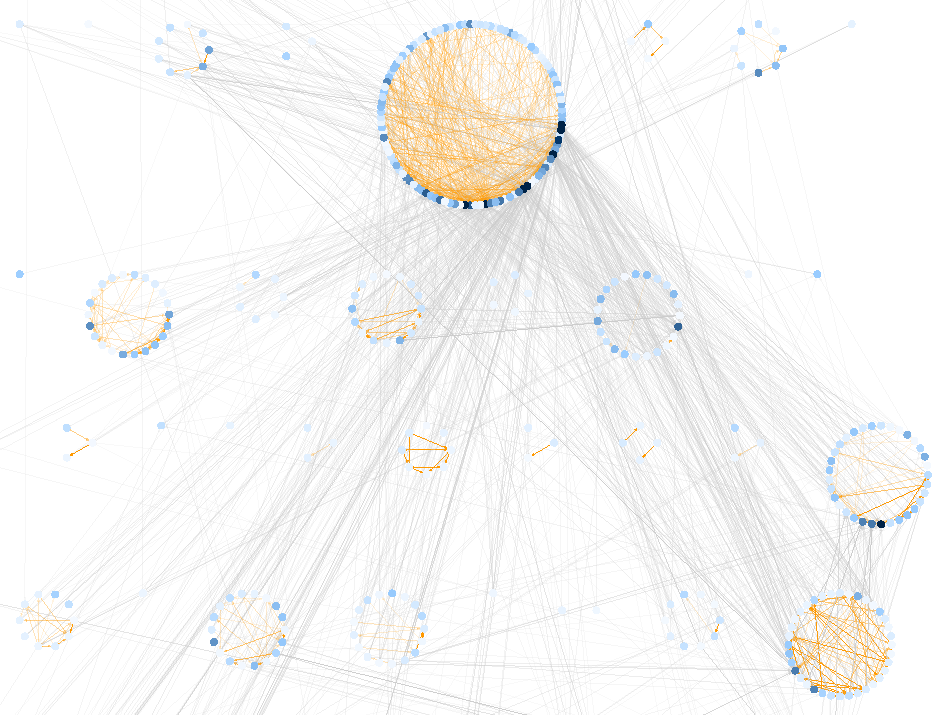
\includegraphics[width=\columnwidth]{Figs/final-overview.pdf}
    \caption{An example {\em Via} graph, showcasing enrollment
      patterns within different departments. Each ring is comprised of
      courses offered by one department.}
    \label{fig:overview}
\end{figure}
Tool users can zoom to select particular courses or
departments. The selections can then be extracted as a separate
graph. These interactions are implemented by \textit{Cytoscape}, which
we use as the engine behind {\em Via} \cite{shannon2003cytoscape}.

Cytoscape was developed to model biological systems and interactions
between cellular organisms. Yet the tool is well suited for
representing our academic pathway data.

Cytoscape uses a spring-embedder system for optimally spacing and
aggregating nodes, and additionally allows the tool operator to
cluster nodes by attributes \cite{Battista1994}. For our purposes, we
display courses within departments as ring structures. For example,
the large ring in Figure \ref{fig:overview} represents the Computer
Science department in a graph generated from enrollment data filtered
to include only CS majors. Each of the dots that comprise the
circumference of the ring is one course in that department. The
interior connecting arrows display the flow of students from one CS
course to another. Links between rings are enrollments of CS majors in
other departments' courses.

{\em Via} assigns unique colorings for both courses (nodes) and
enrollment probabilities (edges) to visualize course and
enrollment-level attributes. In all of the figures below, we color
edges between courses in the same department orange, and all edges
between courses in different departments grey. We further modulate the
thickness of an edge from course \textit{i} to course \textit{j} to
represent the conditional probability of taking course j after course
i. Finally, each node is colored in a blue-gradient, representing the
prior probability of a student enrolling in the respective course. For
example, a deep blue node would be a course that many students are
highly likely to enroll in during their undergraduate years.

Note that while a {\em Via} graph {\em aggregates} all students---no
single student's information is represented---we can choose to make
available to {\em Via} only students with certain characteristics. In
Figure~\ref{fig:overview} this attribute is {\em major}. We could as
easily construct such overviews that distinguish between, for example,
gender or minority status.

Beyond visualizations {\em Via} provides a second, more formal avenue
for analysis. Because the tool's principle visual element is a graph, many
graph related mathematical approaches are available. These include
variations of centrality and betweenness, clustering, Page Rank, and
others. Applications in the following section will exemplify the use
of the visual methods. Section~\secref{sec:advanced} will add
applications that use graph computations.
